% Options for packages loaded elsewhere
\PassOptionsToPackage{unicode}{hyperref}
\PassOptionsToPackage{hyphens}{url}
%
\documentclass[
]{article}
\title{Class17 Vax Mini Project}
\author{Monica Lin (PID: A15524235)}
\date{11/25/2021}

\usepackage{amsmath,amssymb}
\usepackage{lmodern}
\usepackage{iftex}
\ifPDFTeX
  \usepackage[T1]{fontenc}
  \usepackage[utf8]{inputenc}
  \usepackage{textcomp} % provide euro and other symbols
\else % if luatex or xetex
  \usepackage{unicode-math}
  \defaultfontfeatures{Scale=MatchLowercase}
  \defaultfontfeatures[\rmfamily]{Ligatures=TeX,Scale=1}
\fi
% Use upquote if available, for straight quotes in verbatim environments
\IfFileExists{upquote.sty}{\usepackage{upquote}}{}
\IfFileExists{microtype.sty}{% use microtype if available
  \usepackage[]{microtype}
  \UseMicrotypeSet[protrusion]{basicmath} % disable protrusion for tt fonts
}{}
\makeatletter
\@ifundefined{KOMAClassName}{% if non-KOMA class
  \IfFileExists{parskip.sty}{%
    \usepackage{parskip}
  }{% else
    \setlength{\parindent}{0pt}
    \setlength{\parskip}{6pt plus 2pt minus 1pt}}
}{% if KOMA class
  \KOMAoptions{parskip=half}}
\makeatother
\usepackage{xcolor}
\IfFileExists{xurl.sty}{\usepackage{xurl}}{} % add URL line breaks if available
\IfFileExists{bookmark.sty}{\usepackage{bookmark}}{\usepackage{hyperref}}
\hypersetup{
  pdftitle={Class17 Vax Mini Project},
  pdfauthor={Monica Lin (PID: A15524235)},
  hidelinks,
  pdfcreator={LaTeX via pandoc}}
\urlstyle{same} % disable monospaced font for URLs
\usepackage[margin=1in]{geometry}
\usepackage{color}
\usepackage{fancyvrb}
\newcommand{\VerbBar}{|}
\newcommand{\VERB}{\Verb[commandchars=\\\{\}]}
\DefineVerbatimEnvironment{Highlighting}{Verbatim}{commandchars=\\\{\}}
% Add ',fontsize=\small' for more characters per line
\usepackage{framed}
\definecolor{shadecolor}{RGB}{248,248,248}
\newenvironment{Shaded}{\begin{snugshade}}{\end{snugshade}}
\newcommand{\AlertTok}[1]{\textcolor[rgb]{0.94,0.16,0.16}{#1}}
\newcommand{\AnnotationTok}[1]{\textcolor[rgb]{0.56,0.35,0.01}{\textbf{\textit{#1}}}}
\newcommand{\AttributeTok}[1]{\textcolor[rgb]{0.77,0.63,0.00}{#1}}
\newcommand{\BaseNTok}[1]{\textcolor[rgb]{0.00,0.00,0.81}{#1}}
\newcommand{\BuiltInTok}[1]{#1}
\newcommand{\CharTok}[1]{\textcolor[rgb]{0.31,0.60,0.02}{#1}}
\newcommand{\CommentTok}[1]{\textcolor[rgb]{0.56,0.35,0.01}{\textit{#1}}}
\newcommand{\CommentVarTok}[1]{\textcolor[rgb]{0.56,0.35,0.01}{\textbf{\textit{#1}}}}
\newcommand{\ConstantTok}[1]{\textcolor[rgb]{0.00,0.00,0.00}{#1}}
\newcommand{\ControlFlowTok}[1]{\textcolor[rgb]{0.13,0.29,0.53}{\textbf{#1}}}
\newcommand{\DataTypeTok}[1]{\textcolor[rgb]{0.13,0.29,0.53}{#1}}
\newcommand{\DecValTok}[1]{\textcolor[rgb]{0.00,0.00,0.81}{#1}}
\newcommand{\DocumentationTok}[1]{\textcolor[rgb]{0.56,0.35,0.01}{\textbf{\textit{#1}}}}
\newcommand{\ErrorTok}[1]{\textcolor[rgb]{0.64,0.00,0.00}{\textbf{#1}}}
\newcommand{\ExtensionTok}[1]{#1}
\newcommand{\FloatTok}[1]{\textcolor[rgb]{0.00,0.00,0.81}{#1}}
\newcommand{\FunctionTok}[1]{\textcolor[rgb]{0.00,0.00,0.00}{#1}}
\newcommand{\ImportTok}[1]{#1}
\newcommand{\InformationTok}[1]{\textcolor[rgb]{0.56,0.35,0.01}{\textbf{\textit{#1}}}}
\newcommand{\KeywordTok}[1]{\textcolor[rgb]{0.13,0.29,0.53}{\textbf{#1}}}
\newcommand{\NormalTok}[1]{#1}
\newcommand{\OperatorTok}[1]{\textcolor[rgb]{0.81,0.36,0.00}{\textbf{#1}}}
\newcommand{\OtherTok}[1]{\textcolor[rgb]{0.56,0.35,0.01}{#1}}
\newcommand{\PreprocessorTok}[1]{\textcolor[rgb]{0.56,0.35,0.01}{\textit{#1}}}
\newcommand{\RegionMarkerTok}[1]{#1}
\newcommand{\SpecialCharTok}[1]{\textcolor[rgb]{0.00,0.00,0.00}{#1}}
\newcommand{\SpecialStringTok}[1]{\textcolor[rgb]{0.31,0.60,0.02}{#1}}
\newcommand{\StringTok}[1]{\textcolor[rgb]{0.31,0.60,0.02}{#1}}
\newcommand{\VariableTok}[1]{\textcolor[rgb]{0.00,0.00,0.00}{#1}}
\newcommand{\VerbatimStringTok}[1]{\textcolor[rgb]{0.31,0.60,0.02}{#1}}
\newcommand{\WarningTok}[1]{\textcolor[rgb]{0.56,0.35,0.01}{\textbf{\textit{#1}}}}
\usepackage{longtable,booktabs,array}
\usepackage{calc} % for calculating minipage widths
% Correct order of tables after \paragraph or \subparagraph
\usepackage{etoolbox}
\makeatletter
\patchcmd\longtable{\par}{\if@noskipsec\mbox{}\fi\par}{}{}
\makeatother
% Allow footnotes in longtable head/foot
\IfFileExists{footnotehyper.sty}{\usepackage{footnotehyper}}{\usepackage{footnote}}
\makesavenoteenv{longtable}
\usepackage{graphicx}
\makeatletter
\def\maxwidth{\ifdim\Gin@nat@width>\linewidth\linewidth\else\Gin@nat@width\fi}
\def\maxheight{\ifdim\Gin@nat@height>\textheight\textheight\else\Gin@nat@height\fi}
\makeatother
% Scale images if necessary, so that they will not overflow the page
% margins by default, and it is still possible to overwrite the defaults
% using explicit options in \includegraphics[width, height, ...]{}
\setkeys{Gin}{width=\maxwidth,height=\maxheight,keepaspectratio}
% Set default figure placement to htbp
\makeatletter
\def\fps@figure{htbp}
\makeatother
\setlength{\emergencystretch}{3em} % prevent overfull lines
\providecommand{\tightlist}{%
  \setlength{\itemsep}{0pt}\setlength{\parskip}{0pt}}
\setcounter{secnumdepth}{-\maxdimen} % remove section numbering
\ifLuaTeX
  \usepackage{selnolig}  % disable illegal ligatures
\fi

\begin{document}
\maketitle

\hypertarget{background}{%
\section{Background}\label{background}}

The goal of this hands-on mini-project is to examine and compare the
Covid-19 vaccination rates around San Diego.

We will start by downloading the most recently dated ``Statewide
COVID-19 Vaccines Administered by ZIP Code'' CSV file from:
\url{https://data.ca.gov/dataset/covid-19-vaccine-progress-dashboard-data-by-zip-code}

Move the downloaded CSV file to the Class17 project directory, then
read/import into an R object named \texttt{vax}. Use this data to answer
all the questions below.

\begin{Shaded}
\begin{Highlighting}[]
\CommentTok{\# Import vaccination data}
\NormalTok{vax }\OtherTok{\textless{}{-}} \FunctionTok{read.csv}\NormalTok{(}\StringTok{"covid19vaccinesbyzipcode\_test.csv"}\NormalTok{)}
\FunctionTok{head}\NormalTok{(vax)}
\end{Highlighting}
\end{Shaded}

\begin{verbatim}
##   as_of_date zip_code_tabulation_area local_health_jurisdiction         county
## 1 2021-01-05                    92395            San Bernardino San Bernardino
## 2 2021-01-05                    93206                      Kern           Kern
## 3 2021-01-05                    91006               Los Angeles    Los Angeles
## 4 2021-01-05                    91901                 San Diego      San Diego
## 5 2021-01-05                    92230                 Riverside      Riverside
## 6 2021-01-05                    92662                    Orange         Orange
##   vaccine_equity_metric_quartile                 vem_source
## 1                              1 Healthy Places Index Score
## 2                              1 Healthy Places Index Score
## 3                              3 Healthy Places Index Score
## 4                              3 Healthy Places Index Score
## 5                              1 Healthy Places Index Score
## 6                              4 Healthy Places Index Score
##   age12_plus_population age5_plus_population persons_fully_vaccinated
## 1               35915.3                40888                       NA
## 2                1237.5                 1521                       NA
## 3               28742.7                31347                       19
## 4               15549.8                16905                       12
## 5                2320.2                 2526                       NA
## 6                2349.5                 2397                       NA
##   persons_partially_vaccinated percent_of_population_fully_vaccinated
## 1                           NA                                     NA
## 2                           NA                                     NA
## 3                          873                               0.000606
## 4                          271                               0.000710
## 5                           NA                                     NA
## 6                           NA                                     NA
##   percent_of_population_partially_vaccinated
## 1                                         NA
## 2                                         NA
## 3                                   0.027850
## 4                                   0.016031
## 5                                         NA
## 6                                         NA
##   percent_of_population_with_1_plus_dose
## 1                                     NA
## 2                                     NA
## 3                               0.028456
## 4                               0.016741
## 5                                     NA
## 6                                     NA
##                                                                redacted
## 1 Information redacted in accordance with CA state privacy requirements
## 2 Information redacted in accordance with CA state privacy requirements
## 3                                                                    No
## 4                                                                    No
## 5 Information redacted in accordance with CA state privacy requirements
## 6 Information redacted in accordance with CA state privacy requirements
\end{verbatim}

\begin{quote}
\textbf{Q1}. What column details the total number of people fully
vaccinated?
\end{quote}

The column ``persons\_fully\_vaccinated'' details the total number of
people fully vaccinated.

\begin{quote}
\textbf{Q2}. What column details the Zip code tabulation area?
\end{quote}

``zip\_code\_tabulation\_area''.

\begin{quote}
\textbf{Q3}. What is the earliest date in this dataset?
\end{quote}

\begin{Shaded}
\begin{Highlighting}[]
\FunctionTok{head}\NormalTok{(vax}\SpecialCharTok{$}\NormalTok{as\_of\_date)}
\end{Highlighting}
\end{Shaded}

\begin{verbatim}
## [1] "2021-01-05" "2021-01-05" "2021-01-05" "2021-01-05" "2021-01-05"
## [6] "2021-01-05"
\end{verbatim}

The earliest date in the dataset is 2021-01-05, by Year-month-date.

\begin{quote}
\textbf{Q4}. What is the latest date in this dataset?
\end{quote}

\begin{Shaded}
\begin{Highlighting}[]
\FunctionTok{tail}\NormalTok{(vax}\SpecialCharTok{$}\NormalTok{as\_of\_date)}
\end{Highlighting}
\end{Shaded}

\begin{verbatim}
## [1] "2021-11-23" "2021-11-23" "2021-11-23" "2021-11-23" "2021-11-23"
## [6] "2021-11-23"
\end{verbatim}

The latest date in this dataset is 2021-11-23.

Let's call the \texttt{skim()} function from the \textbf{skimr} package
to get a quick overview of this dataset.

\begin{Shaded}
\begin{Highlighting}[]
\FunctionTok{library}\NormalTok{(skimr)}
\NormalTok{skimr}\SpecialCharTok{::}\FunctionTok{skim}\NormalTok{(vax)}
\end{Highlighting}
\end{Shaded}

\begin{longtable}[]{@{}ll@{}}
\caption{Data summary}\tabularnewline
\toprule
\endhead
Name & vax \\
Number of rows & 82908 \\
Number of columns & 14 \\
\_\_\_\_\_\_\_\_\_\_\_\_\_\_\_\_\_\_\_\_\_\_\_ & \\
Column type frequency: & \\
character & 5 \\
numeric & 9 \\
\_\_\_\_\_\_\_\_\_\_\_\_\_\_\_\_\_\_\_\_\_\_\_\_ & \\
Group variables & None \\
\bottomrule
\end{longtable}

\textbf{Variable type: character}

\begin{longtable}[]{@{}lrrrrrrr@{}}
\toprule
skim\_variable & n\_missing & complete\_rate & min & max & empty &
n\_unique & whitespace \\
\midrule
\endhead
as\_of\_date & 0 & 1 & 10 & 10 & 0 & 47 & 0 \\
local\_health\_jurisdiction & 0 & 1 & 0 & 15 & 235 & 62 & 0 \\
county & 0 & 1 & 0 & 15 & 235 & 59 & 0 \\
vem\_source & 0 & 1 & 15 & 26 & 0 & 3 & 0 \\
redacted & 0 & 1 & 2 & 69 & 0 & 2 & 0 \\
\bottomrule
\end{longtable}

\textbf{Variable type: numeric}

\begin{longtable}[]{@{}
  >{\raggedright\arraybackslash}p{(\columnwidth - 20\tabcolsep) * \real{0.26}}
  >{\raggedleft\arraybackslash}p{(\columnwidth - 20\tabcolsep) * \real{0.06}}
  >{\raggedleft\arraybackslash}p{(\columnwidth - 20\tabcolsep) * \real{0.08}}
  >{\raggedleft\arraybackslash}p{(\columnwidth - 20\tabcolsep) * \real{0.05}}
  >{\raggedleft\arraybackslash}p{(\columnwidth - 20\tabcolsep) * \real{0.05}}
  >{\raggedleft\arraybackslash}p{(\columnwidth - 20\tabcolsep) * \real{0.04}}
  >{\raggedleft\arraybackslash}p{(\columnwidth - 20\tabcolsep) * \real{0.05}}
  >{\raggedleft\arraybackslash}p{(\columnwidth - 20\tabcolsep) * \real{0.05}}
  >{\raggedleft\arraybackslash}p{(\columnwidth - 20\tabcolsep) * \real{0.05}}
  >{\raggedleft\arraybackslash}p{(\columnwidth - 20\tabcolsep) * \real{0.05}}
  >{\raggedright\arraybackslash}p{(\columnwidth - 20\tabcolsep) * \real{0.24}}@{}}
\toprule
\begin{minipage}[b]{\linewidth}\raggedright
skim\_variable
\end{minipage} & \begin{minipage}[b]{\linewidth}\raggedleft
n\_missing
\end{minipage} & \begin{minipage}[b]{\linewidth}\raggedleft
complete\_rate
\end{minipage} & \begin{minipage}[b]{\linewidth}\raggedleft
mean
\end{minipage} & \begin{minipage}[b]{\linewidth}\raggedleft
sd
\end{minipage} & \begin{minipage}[b]{\linewidth}\raggedleft
p0
\end{minipage} & \begin{minipage}[b]{\linewidth}\raggedleft
p25
\end{minipage} & \begin{minipage}[b]{\linewidth}\raggedleft
p50
\end{minipage} & \begin{minipage}[b]{\linewidth}\raggedleft
p75
\end{minipage} & \begin{minipage}[b]{\linewidth}\raggedleft
p100
\end{minipage} & \begin{minipage}[b]{\linewidth}\raggedright
hist
\end{minipage} \\
\midrule
\endhead
zip\_code\_tabulation\_area & 0 & 1.00 & 93665.11 & 1817.39 & 90001 &
92257.75 & 93658.50 & 95380.50 & 97635.0 & ▃▅▅▇▁ \\
vaccine\_equity\_metric\_quartile & 4089 & 0.95 & 2.44 & 1.11 & 1 & 1.00
& 2.00 & 3.00 & 4.0 & ▇▇▁▇▇ \\
age12\_plus\_population & 0 & 1.00 & 18895.04 & 18993.94 & 0 & 1346.95 &
13685.10 & 31756.12 & 88556.7 & ▇▃▂▁▁ \\
age5\_plus\_population & 0 & 1.00 & 20875.24 & 21106.04 & 0 & 1460.50 &
15364.00 & 34877.00 & 101902.0 & ▇▃▂▁▁ \\
persons\_fully\_vaccinated & 8355 & 0.90 & 9585.35 & 11609.12 & 11 &
516.00 & 4210.00 & 16095.00 & 71219.0 & ▇▂▁▁▁ \\
persons\_partially\_vaccinated & 8355 & 0.90 & 1894.87 & 2105.55 & 11 &
198.00 & 1269.00 & 2880.00 & 20159.0 & ▇▁▁▁▁ \\
percent\_of\_population\_fully\_vaccinated & 8355 & 0.90 & 0.43 & 0.27 &
0 & 0.20 & 0.44 & 0.63 & 1.0 & ▇▆▇▆▂ \\
percent\_of\_population\_partially\_vaccinated & 8355 & 0.90 & 0.10 &
0.10 & 0 & 0.06 & 0.07 & 0.11 & 1.0 & ▇▁▁▁▁ \\
percent\_of\_population\_with\_1\_plus\_dose & 8355 & 0.90 & 0.51 & 0.26
& 0 & 0.31 & 0.53 & 0.71 & 1.0 & ▅▅▇▇▃ \\
\bottomrule
\end{longtable}

\begin{quote}
\textbf{Q5}. How many numeric columns are in this dataset?
\end{quote}

9

\begin{quote}
\textbf{Q6}. Note that there are ``missing values'' in the dataset. How
many \texttt{NA} values are there in the
\texttt{persons\_fully\_vaccinated} column?
\end{quote}

\begin{Shaded}
\begin{Highlighting}[]
\FunctionTok{sum}\NormalTok{( }\FunctionTok{is.na}\NormalTok{(vax}\SpecialCharTok{$}\NormalTok{persons\_fully\_vaccinated) )}
\end{Highlighting}
\end{Shaded}

\begin{verbatim}
## [1] 8355
\end{verbatim}

There are 8355 NA values in that column.

\begin{quote}
\textbf{Q7}. What percent of \texttt{persons\_fully\_vaccinated} values
are missing (to two significant figures)?
\end{quote}

\begin{Shaded}
\begin{Highlighting}[]
\FunctionTok{sum}\NormalTok{( }\FunctionTok{is.na}\NormalTok{(vax}\SpecialCharTok{$}\NormalTok{persons\_fully\_vaccinated) ) }\SpecialCharTok{/} \FunctionTok{nrow}\NormalTok{(vax)}
\end{Highlighting}
\end{Shaded}

\begin{verbatim}
## [1] 0.1007744
\end{verbatim}

10.08\% of \texttt{persons\_fully\_vaccinated} values are missing.

\begin{quote}
\textbf{Q8}. {[}Optional{]}: Why might this data be missing?
\end{quote}

Optional.

\hypertarget{working-with-dates}{%
\section{Working with dates}\label{working-with-dates}}

One of the ``character'' columns of the data is \texttt{as\_of\_date},
which contains dates in the Year-Month-Day format.

Dates and times can be annoying to work with at the best of times.
However, in R we have the excellent \textbf{lubridate} package, which
makes life a lot easier when dealing with dates and times. Here is a
quick example to get you started:

\begin{Shaded}
\begin{Highlighting}[]
\CommentTok{\# install.packages("lubridate")}
\FunctionTok{library}\NormalTok{(lubridate)}
\end{Highlighting}
\end{Shaded}

\begin{verbatim}
## Warning: package 'lubridate' was built under R version 4.1.2
\end{verbatim}

\begin{verbatim}
## 
## Attaching package: 'lubridate'
\end{verbatim}

\begin{verbatim}
## The following objects are masked from 'package:base':
## 
##     date, intersect, setdiff, union
\end{verbatim}

What is today's date?

\begin{Shaded}
\begin{Highlighting}[]
\FunctionTok{today}\NormalTok{()}
\end{Highlighting}
\end{Shaded}

\begin{verbatim}
## [1] "2021-11-27"
\end{verbatim}

The \texttt{as\_of\_date} column of our data is currently not that
usable. For example, we can't easily do math with it like answering the
simple question of how many days have passed since data was first
recorded:

However, if we convert our date data into a lubridate format, this like
this will be much easier (as well as plotting time series data later
on).

\begin{Shaded}
\begin{Highlighting}[]
\CommentTok{\# Specify that we are using the Year{-}month{-}day format}
\NormalTok{vax}\SpecialCharTok{$}\NormalTok{as\_of\_date }\OtherTok{\textless{}{-}} \FunctionTok{ymd}\NormalTok{(vax}\SpecialCharTok{$}\NormalTok{as\_of\_date)}
\end{Highlighting}
\end{Shaded}

Now we can do math with dates. For example: How mnay days have passed
since the first vaccination reported in this dataset?

\begin{Shaded}
\begin{Highlighting}[]
\FunctionTok{today}\NormalTok{() }\SpecialCharTok{{-}}\NormalTok{ vax}\SpecialCharTok{$}\NormalTok{as\_of\_date[}\DecValTok{1}\NormalTok{]}
\end{Highlighting}
\end{Shaded}

\begin{verbatim}
## Time difference of 326 days
\end{verbatim}

Using the last and the first date value, we can now determine how many
days the dataset span.

\begin{Shaded}
\begin{Highlighting}[]
\NormalTok{vax}\SpecialCharTok{$}\NormalTok{as\_of\_date[}\FunctionTok{nrow}\NormalTok{(vax)] }\SpecialCharTok{{-}}\NormalTok{ vax}\SpecialCharTok{$}\NormalTok{as\_of\_date[}\DecValTok{1}\NormalTok{]}
\end{Highlighting}
\end{Shaded}

\begin{verbatim}
## Time difference of 322 days
\end{verbatim}

\begin{quote}
\textbf{Q9}. How many days have passed since the last update of the
dataset?
\end{quote}

\begin{Shaded}
\begin{Highlighting}[]
\FunctionTok{today}\NormalTok{() }\SpecialCharTok{{-}}\NormalTok{ vax}\SpecialCharTok{$}\NormalTok{as\_of\_date[}\FunctionTok{nrow}\NormalTok{(vax)]}
\end{Highlighting}
\end{Shaded}

\begin{verbatim}
## Time difference of 4 days
\end{verbatim}

It has been 4 days since the last entry.

\begin{quote}
\textbf{Q10}. How many unique dates are in the dataset (i.e.~how many
different dates are detailed?)
\end{quote}

\begin{Shaded}
\begin{Highlighting}[]
\FunctionTok{length}\NormalTok{(}\FunctionTok{unique}\NormalTok{(vax}\SpecialCharTok{$}\NormalTok{as\_of\_date))}
\end{Highlighting}
\end{Shaded}

\begin{verbatim}
## [1] 47
\end{verbatim}

There are 47 unique dates in the dataset.

\hypertarget{working-with-zip-codes}{%
\section{Working with ZIP codes}\label{working-with-zip-codes}}

One of the numeric columns in the dataset (namely
\texttt{vax\$zip\_code\_tabulation\_area}) are actually ZIP codes -- a
postal code used by the United States Postal Service (USPS). In R, we
can use the \textbf{zipcodeR} package to make working with these codes
easier. For example, let's install and thn load up this package to find
the centroid of the La Jolla 92037 (i.e.~UC San Diego) ZIP code area.

\begin{Shaded}
\begin{Highlighting}[]
\CommentTok{\# install.packages("zipcodeR")}
\FunctionTok{library}\NormalTok{(zipcodeR)}
\end{Highlighting}
\end{Shaded}

\begin{verbatim}
## Warning: package 'zipcodeR' was built under R version 4.1.2
\end{verbatim}

\begin{Shaded}
\begin{Highlighting}[]
\CommentTok{\# Find centroid of La Jolla 92037 ZIP code area}
\FunctionTok{geocode\_zip}\NormalTok{(}\StringTok{\textquotesingle{}92037\textquotesingle{}}\NormalTok{)}
\end{Highlighting}
\end{Shaded}

\begin{verbatim}
## # A tibble: 1 x 3
##   zipcode   lat   lng
##   <chr>   <dbl> <dbl>
## 1 92037    32.8 -117.
\end{verbatim}

Calculate the distance between the centroids of any two ZIP codes in
miles, e.g.

\begin{Shaded}
\begin{Highlighting}[]
\FunctionTok{zip\_distance}\NormalTok{(}\StringTok{\textquotesingle{}92037\textquotesingle{}}\NormalTok{, }\StringTok{\textquotesingle{}92109\textquotesingle{}}\NormalTok{)}
\end{Highlighting}
\end{Shaded}

\begin{verbatim}
##   zipcode_a zipcode_b distance
## 1     92037     92109     2.33
\end{verbatim}

More usefully, we can pull census data about ZIP code areas (including
median household income, etc.) For example:

\begin{Shaded}
\begin{Highlighting}[]
\FunctionTok{reverse\_zipcode}\NormalTok{(}\FunctionTok{c}\NormalTok{(}\StringTok{\textquotesingle{}92037\textquotesingle{}}\NormalTok{, }\StringTok{\textquotesingle{}92109\textquotesingle{}}\NormalTok{))}
\end{Highlighting}
\end{Shaded}

\begin{verbatim}
## # A tibble: 2 x 24
##   zipcode zipcode_type major_city post_office_city common_city_list county state
##   <chr>   <chr>        <chr>      <chr>                      <blob> <chr>  <chr>
## 1 92037   Standard     La Jolla   La Jolla, CA           <raw 20 B> San D~ CA   
## 2 92109   Standard     San Diego  San Diego, CA          <raw 21 B> San D~ CA   
## # ... with 17 more variables: lat <dbl>, lng <dbl>, timezone <chr>,
## #   radius_in_miles <dbl>, area_code_list <blob>, population <int>,
## #   population_density <dbl>, land_area_in_sqmi <dbl>,
## #   water_area_in_sqmi <dbl>, housing_units <int>,
## #   occupied_housing_units <int>, median_home_value <int>,
## #   median_household_income <int>, bounds_west <dbl>, bounds_east <dbl>,
## #   bounds_north <dbl>, bounds_south <dbl>
\end{verbatim}

We can use this \texttt{reverse\_zipcode()} to pull census data later on
for any or all ZIP code areas we might be interested in.

\begin{Shaded}
\begin{Highlighting}[]
\CommentTok{\# Pull data for all ZIP codes in the dataset}
\NormalTok{zipdata }\OtherTok{\textless{}{-}} \FunctionTok{reverse\_zipcode}\NormalTok{( vax}\SpecialCharTok{$}\NormalTok{zip\_code\_tabulation\_area)}
\end{Highlighting}
\end{Shaded}

\hypertarget{focus-on-the-san-diego-area}{%
\section{Focus on the San Diego
area}\label{focus-on-the-san-diego-area}}

Let's now focus in on the San Diego County area by restricting ourselves
first to \texttt{vax\$county\ ==\ "San\ Diego"} entries. We have two
main choices on how to do this: the first using base R, the second using
the \textbf{dplyr} package:

\begin{Shaded}
\begin{Highlighting}[]
\FunctionTok{table}\NormalTok{(vax}\SpecialCharTok{$}\NormalTok{county)}
\end{Highlighting}
\end{Shaded}

\begin{verbatim}
## 
##                         Alameda          Alpine          Amador           Butte 
##             235            2303              47             564             846 
##       Calaveras          Colusa    Contra Costa       Del Norte       El Dorado 
##             846             329            2021             188            1034 
##          Fresno           Glenn        Humboldt        Imperial            Inyo 
##            2585             282            1645             705             470 
##            Kern           Kings            Lake          Lassen     Los Angeles 
##            2303             329             658             611           13630 
##          Madera           Marin        Mariposa       Mendocino          Merced 
##             564            1316             376            1222             893 
##           Modoc            Mono        Monterey            Napa          Nevada 
##             517             329            1316             470             564 
##          Orange          Placer          Plumas       Riverside      Sacramento 
##            4136            1363             752            3290            2538 
##      San Benito  San Bernardino       San Diego   San Francisco     San Joaquin 
##             188            4183            5029            1269            1504 
## San Luis Obispo       San Mateo   Santa Barbara     Santa Clara      Santa Cruz 
##            1034            1363            1081            2726             799 
##          Shasta          Sierra        Siskiyou          Solano          Sonoma 
##            1222             329             987             705            1692 
##      Stanislaus          Sutter          Tehama         Trinity          Tulare 
##            1128             423             611             611            1551 
##        Tuolumne         Ventura            Yolo            Yuba 
##             611            1269             799             517
\end{verbatim}

\begin{Shaded}
\begin{Highlighting}[]
\NormalTok{inds }\OtherTok{\textless{}{-}}\NormalTok{ vax}\SpecialCharTok{$}\NormalTok{county}\SpecialCharTok{==}\StringTok{"San Diego"}
\FunctionTok{head}\NormalTok{(vax[inds, ])}
\end{Highlighting}
\end{Shaded}

\begin{verbatim}
##    as_of_date zip_code_tabulation_area local_health_jurisdiction    county
## 4  2021-01-05                    91901                 San Diego San Diego
## 14 2021-01-05                    91902                 San Diego San Diego
## 21 2021-01-05                    92011                 San Diego San Diego
## 22 2021-01-05                    92055                 San Diego San Diego
## 25 2021-01-05                    92067                 San Diego San Diego
## 33 2021-01-05                    92081                 San Diego San Diego
##    vaccine_equity_metric_quartile                 vem_source
## 4                               3 Healthy Places Index Score
## 14                              4 Healthy Places Index Score
## 21                              4 Healthy Places Index Score
## 22                              3    CDPH-Derived ZCTA Score
## 25                              4 Healthy Places Index Score
## 33                              2 Healthy Places Index Score
##    age12_plus_population age5_plus_population persons_fully_vaccinated
## 4                15549.8                16905                       12
## 14               16620.7                18026                       22
## 21               20503.6                23247                       NA
## 22               11548.0                11654                       NA
## 25                6973.9                 7480                       11
## 33               25558.0                27632                       14
##    persons_partially_vaccinated percent_of_population_fully_vaccinated
## 4                           271                               0.000710
## 14                          374                               0.001220
## 21                           NA                                     NA
## 22                           NA                                     NA
## 25                          241                               0.001471
## 33                          346                               0.000507
##    percent_of_population_partially_vaccinated
## 4                                    0.016031
## 14                                   0.020748
## 21                                         NA
## 22                                         NA
## 25                                   0.032219
## 33                                   0.012522
##    percent_of_population_with_1_plus_dose
## 4                                0.016741
## 14                               0.021968
## 21                                     NA
## 22                                     NA
## 25                               0.033690
## 33                               0.013029
##                                                                 redacted
## 4                                                                     No
## 14                                                                    No
## 21 Information redacted in accordance with CA state privacy requirements
## 22 Information redacted in accordance with CA state privacy requirements
## 25                                                                    No
## 33                                                                    No
\end{verbatim}

Using the \textbf{dplyr} package and its \textbf{filter()} function, the
code would look like this:

\begin{Shaded}
\begin{Highlighting}[]
\FunctionTok{library}\NormalTok{(dplyr)}
\end{Highlighting}
\end{Shaded}

\begin{verbatim}
## 
## Attaching package: 'dplyr'
\end{verbatim}

\begin{verbatim}
## The following objects are masked from 'package:stats':
## 
##     filter, lag
\end{verbatim}

\begin{verbatim}
## The following objects are masked from 'package:base':
## 
##     intersect, setdiff, setequal, union
\end{verbatim}

\begin{Shaded}
\begin{Highlighting}[]
\NormalTok{sd }\OtherTok{\textless{}{-}} \FunctionTok{filter}\NormalTok{(vax, county }\SpecialCharTok{==} \StringTok{"San Diego"}\NormalTok{)}

\FunctionTok{nrow}\NormalTok{(sd)}
\end{Highlighting}
\end{Shaded}

\begin{verbatim}
## [1] 5029
\end{verbatim}

Using \textbf{dplyr} is often more convenient when we are subsetting
across multiple criteria -- for example, all San Diego county areas with
a population of over 10,000.

\begin{Shaded}
\begin{Highlighting}[]
\NormalTok{sd}\FloatTok{.10} \OtherTok{\textless{}{-}} \FunctionTok{filter}\NormalTok{(vax, county }\SpecialCharTok{==} \StringTok{"San Diego"} \SpecialCharTok{\&}
\NormalTok{                  age5\_plus\_population }\SpecialCharTok{\textgreater{}} \DecValTok{10000}\NormalTok{)}
\end{Highlighting}
\end{Shaded}

\begin{quote}
\textbf{Q11}. How many distinct zip codes are listed for San Diego
County?
\end{quote}

\begin{Shaded}
\begin{Highlighting}[]
\FunctionTok{length}\NormalTok{(}\FunctionTok{unique}\NormalTok{(sd}\SpecialCharTok{$}\NormalTok{zip\_code\_tabulation\_area))}
\end{Highlighting}
\end{Shaded}

\begin{verbatim}
## [1] 107
\end{verbatim}

There are 107 distinct ZIP codes listed for San Diego County.

\begin{quote}
\textbf{Q12}. What San Diego County zip code area has the largest 12+
Population in this dataset?
\end{quote}

\begin{Shaded}
\begin{Highlighting}[]
\FunctionTok{which.max}\NormalTok{(sd}\SpecialCharTok{$}\NormalTok{age12\_plus\_population)}
\end{Highlighting}
\end{Shaded}

\begin{verbatim}
## [1] 60
\end{verbatim}

\begin{Shaded}
\begin{Highlighting}[]
\NormalTok{sd}\SpecialCharTok{$}\NormalTok{zip\_code\_tabulation\_area[}\DecValTok{23}\NormalTok{]}
\end{Highlighting}
\end{Shaded}

\begin{verbatim}
## [1] 92057
\end{verbatim}

The San Diego County ZIP code area of 92057 has the largest 12+
population in this dataset.

Using \textbf{dplyr}, select all San Diego \emph{``county''} entries on
\emph{``as\_of\_date''} ``2021-11-09'' and use this for the following
questions.

\begin{Shaded}
\begin{Highlighting}[]
\NormalTok{sd.}\FloatTok{11.09} \OtherTok{\textless{}{-}} \FunctionTok{filter}\NormalTok{(vax, county}\SpecialCharTok{==}\StringTok{"San Diego"} \SpecialCharTok{\&}\NormalTok{ as\_of\_date}\SpecialCharTok{==}\StringTok{"2021{-}11{-}09"}\NormalTok{)}
\end{Highlighting}
\end{Shaded}

\begin{quote}
\textbf{Q13}. What is the overall average ``Percent of Population Fully
Vaccinated'' value for all San Diego ``County'' as of ``2021-11-09''?
\end{quote}

\begin{Shaded}
\begin{Highlighting}[]
\FunctionTok{mean}\NormalTok{(sd.}\FloatTok{11.09}\SpecialCharTok{$}\NormalTok{percent\_of\_population\_fully\_vaccinated, }\AttributeTok{na.rm=}\ConstantTok{TRUE}\NormalTok{)}
\end{Highlighting}
\end{Shaded}

\begin{verbatim}
## [1] 0.6734714
\end{verbatim}

The overall average ``Percent of Population Fully Vaccinated'' value is
67.34714\%.

We can look at the 6-number summary.

\begin{Shaded}
\begin{Highlighting}[]
\FunctionTok{summary}\NormalTok{(sd.}\FloatTok{11.09}\SpecialCharTok{$}\NormalTok{percent\_of\_population\_fully\_vaccinated)}
\end{Highlighting}
\end{Shaded}

\begin{verbatim}
##    Min. 1st Qu.  Median    Mean 3rd Qu.    Max.    NA's 
## 0.01017 0.60805 0.67711 0.67347 0.76257 1.00000       4
\end{verbatim}

\begin{quote}
\textbf{Q14}. Using either ggplot or base R graphics, make a summary
figure that show the distribution of Percent of Population Fully
Vaccinated values as of ``2021-11-09''?
\end{quote}

Using base R plots:

\begin{Shaded}
\begin{Highlighting}[]
\FunctionTok{hist}\NormalTok{(sd.}\FloatTok{11.09}\SpecialCharTok{$}\NormalTok{percent\_of\_population\_fully\_vaccinated,}
     \AttributeTok{main=}\StringTok{"Histogram of Vaccination Rates Across San Diego County"}\NormalTok{,}
     \AttributeTok{xlab=}\StringTok{"Percent Fully Vaccinated on 2021{-}11{-}09"}\NormalTok{,}
     \AttributeTok{ylab=}\StringTok{"Frequency"}\NormalTok{)}
\end{Highlighting}
\end{Shaded}

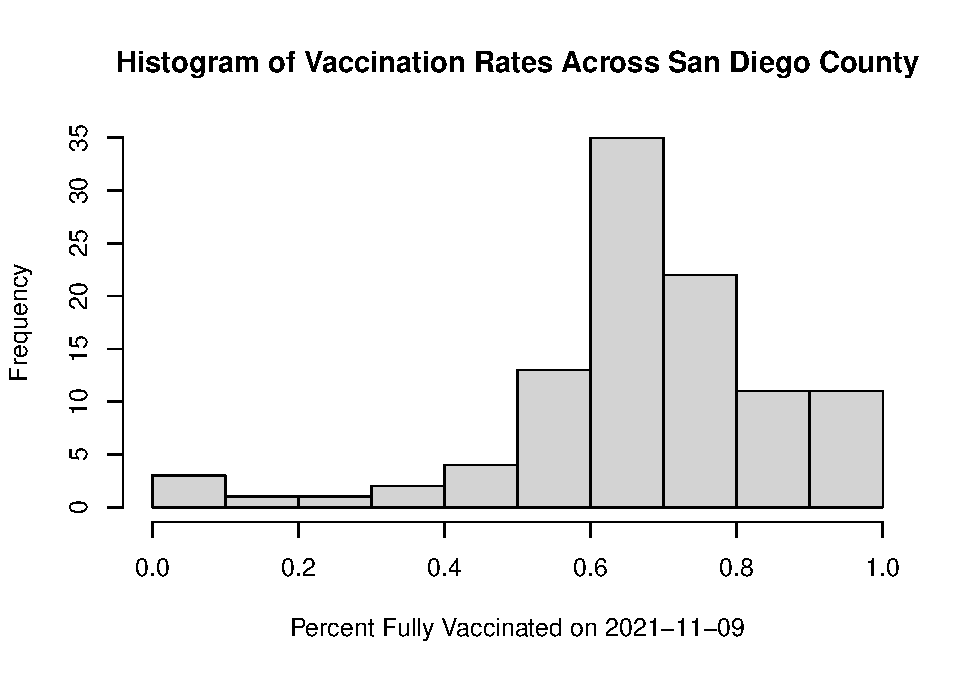
\includegraphics{Class17_files/figure-latex/unnamed-chunk-28-1.pdf}

Using ggplot:

\begin{Shaded}
\begin{Highlighting}[]
\FunctionTok{library}\NormalTok{(ggplot2)}

\FunctionTok{ggplot}\NormalTok{(sd.}\FloatTok{11.09}\NormalTok{) }\SpecialCharTok{+}
  \FunctionTok{aes}\NormalTok{(percent\_of\_population\_fully\_vaccinated) }\SpecialCharTok{+}
  \FunctionTok{geom\_histogram}\NormalTok{(}\AttributeTok{bins=}\DecValTok{10}\NormalTok{) }\SpecialCharTok{+}
  \FunctionTok{labs}\NormalTok{(}\AttributeTok{x=}\StringTok{"Percent Fully Vaccinated on 2021{-}11{-}09"}\NormalTok{, }\AttributeTok{y=}\StringTok{"Count (ZIP Code Areas"}\NormalTok{,}
       \AttributeTok{title=}\StringTok{"Histogram of Vaccination Rates Across San Diego County"}\NormalTok{)}
\end{Highlighting}
\end{Shaded}

\begin{verbatim}
## Warning: Removed 4 rows containing non-finite values (stat_bin).
\end{verbatim}

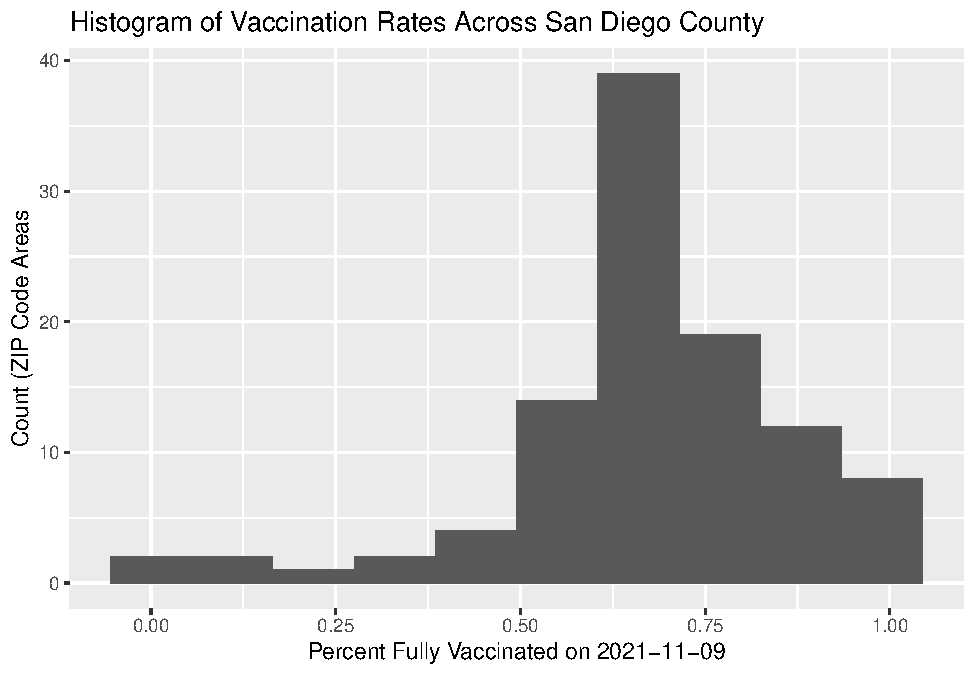
\includegraphics{Class17_files/figure-latex/unnamed-chunk-29-1.pdf}

\hypertarget{focus-on-ucsdla-jolla}{%
\section{Focus on UCSD/La Jolla}\label{focus-on-ucsdla-jolla}}

UC San Diego resides in the 92037 ZIP code area nd is listed with an age
5+ population size of 36,144.

\begin{Shaded}
\begin{Highlighting}[]
\NormalTok{ucsd }\OtherTok{\textless{}{-}} \FunctionTok{filter}\NormalTok{(sd, zip\_code\_tabulation\_area }\SpecialCharTok{==} \StringTok{"92037"}\NormalTok{)}

\NormalTok{ucsd[}\DecValTok{1}\NormalTok{,]}\SpecialCharTok{$}\NormalTok{age5\_plus\_population}
\end{Highlighting}
\end{Shaded}

\begin{verbatim}
## [1] 36144
\end{verbatim}

\begin{quote}
\textbf{Q15}. Using \textbf{ggplot}, make a graph of the vaccination
rate time course for the 92037 ZIP code area:
\end{quote}

\begin{Shaded}
\begin{Highlighting}[]
\FunctionTok{ggplot}\NormalTok{(ucsd) }\SpecialCharTok{+} \FunctionTok{aes}\NormalTok{(as\_of\_date, percent\_of\_population\_fully\_vaccinated) }\SpecialCharTok{+} 
  \FunctionTok{geom\_point}\NormalTok{() }\SpecialCharTok{+} \FunctionTok{geom\_line}\NormalTok{(}\AttributeTok{group=}\DecValTok{1}\NormalTok{) }\SpecialCharTok{+} \FunctionTok{ylim}\NormalTok{(}\FunctionTok{c}\NormalTok{(}\DecValTok{0}\NormalTok{,}\DecValTok{1}\NormalTok{)) }\SpecialCharTok{+}
  \FunctionTok{labs}\NormalTok{(}\AttributeTok{x=}\StringTok{"Date"}\NormalTok{, }\AttributeTok{y=}\StringTok{"Percent Vaccinated"}\NormalTok{, }
       \AttributeTok{title=}\StringTok{"Vaccination Rate for La Jolla CA 92037"}\NormalTok{)}
\end{Highlighting}
\end{Shaded}

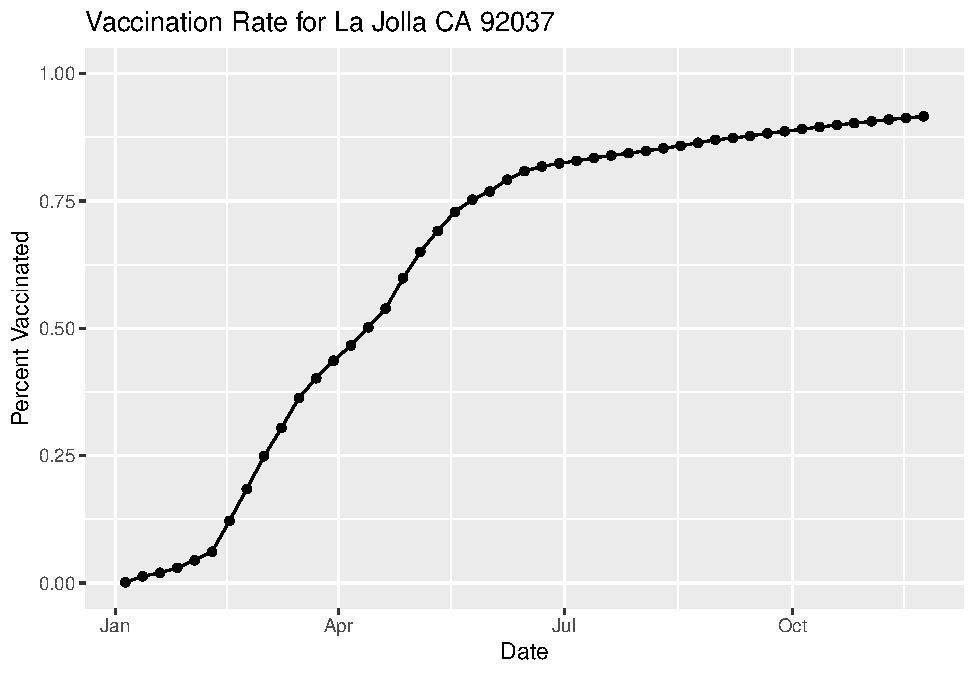
\includegraphics{Class17_files/figure-latex/unnamed-chunk-31-1.pdf}

This plot shows an initial slow roll out in January into Febuary (likely
due to limited vaccine availability). This is followed with rapid ramp
up until a clear slowing trend from June time onward. Interpertation
beyond this requies context from other zip code areas to answer
questions such as: is this trend representative of other areas? Are more
people fully vaccinated in this area compared to others? Etc.

\hypertarget{comparing-92037-to-other-similar-sized-areas}{%
\section{Comparing 92037 to other similar sized
areas}\label{comparing-92037-to-other-similar-sized-areas}}

Let's return to the full dataset and look across every zip code area
with a population at least as large as that of 92037 on
\emph{as\_of\_date} ``2021-11-16''.

\begin{Shaded}
\begin{Highlighting}[]
\CommentTok{\# Subset to all CA areas with a population as large as 92037}
\NormalTok{vax}\FloatTok{.36} \OtherTok{\textless{}{-}} \FunctionTok{filter}\NormalTok{(vax, age5\_plus\_population }\SpecialCharTok{\textgreater{}} \DecValTok{36144} \SpecialCharTok{\&}
\NormalTok{                   as\_of\_date }\SpecialCharTok{==} \StringTok{"2021{-}11{-}16"}\NormalTok{)}

\FunctionTok{head}\NormalTok{(vax}\FloatTok{.36}\NormalTok{)}
\end{Highlighting}
\end{Shaded}

\begin{verbatim}
##   as_of_date zip_code_tabulation_area local_health_jurisdiction         county
## 1 2021-11-16                    92020                 San Diego      San Diego
## 2 2021-11-16                    92563                 Riverside      Riverside
## 3 2021-11-16                    92806                    Orange         Orange
## 4 2021-11-16                    93291                    Tulare         Tulare
## 5 2021-11-16                    92335            San Bernardino San Bernardino
## 6 2021-11-16                    92618                    Orange         Orange
##   vaccine_equity_metric_quartile                 vem_source
## 1                              2 Healthy Places Index Score
## 2                              3 Healthy Places Index Score
## 3                              2 Healthy Places Index Score
## 4                              1 Healthy Places Index Score
## 5                              1 Healthy Places Index Score
## 6                              4 Healthy Places Index Score
##   age12_plus_population age5_plus_population persons_fully_vaccinated
## 1               49284.5                54991                    35128
## 2               55897.8                63794                    36051
## 3               33050.9                36739                    24810
## 4               46879.7                54254                    27936
## 5               79670.3                91867                    49820
## 6               40348.0                44304                    39695
##   persons_partially_vaccinated percent_of_population_fully_vaccinated
## 1                         5161                               0.638795
## 2                         4224                               0.565116
## 3                         2355                               0.675304
## 4                         4012                               0.514911
## 5                         5970                               0.542306
## 6                         3936                               0.895969
##   percent_of_population_partially_vaccinated
## 1                                   0.093852
## 2                                   0.066213
## 3                                   0.064101
## 4                                   0.073948
## 5                                   0.064985
## 6                                   0.088841
##   percent_of_population_with_1_plus_dose redacted
## 1                               0.732647       No
## 2                               0.631329       No
## 3                               0.739405       No
## 4                               0.588859       No
## 5                               0.607291       No
## 6                               0.984810       No
\end{verbatim}

\begin{quote}
\textbf{Q16}. Calculate the mean \emph{``Percent of Population Fully
Vaccinated''} for ZIP code areas with a population as large as 92037 (La
Jolla) \emph{as\_of\_date} ``2021-11-16''. Add this as a straight
horizontal line to your plot from above with the \texttt{geom\_hline()}
function.
\end{quote}

\begin{Shaded}
\begin{Highlighting}[]
\NormalTok{vaccination}\FloatTok{.36} \OtherTok{\textless{}{-}} \FunctionTok{mean}\NormalTok{(vax}\FloatTok{.36}\SpecialCharTok{$}\NormalTok{percent\_of\_population\_fully\_vaccinated)}
\end{Highlighting}
\end{Shaded}

\begin{Shaded}
\begin{Highlighting}[]
\FunctionTok{ggplot}\NormalTok{(ucsd) }\SpecialCharTok{+} \FunctionTok{aes}\NormalTok{(as\_of\_date, percent\_of\_population\_fully\_vaccinated) }\SpecialCharTok{+} 
  \FunctionTok{geom\_point}\NormalTok{() }\SpecialCharTok{+} \FunctionTok{geom\_line}\NormalTok{(}\AttributeTok{group=}\DecValTok{1}\NormalTok{) }\SpecialCharTok{+} \FunctionTok{ylim}\NormalTok{(}\FunctionTok{c}\NormalTok{(}\DecValTok{0}\NormalTok{,}\DecValTok{1}\NormalTok{)) }\SpecialCharTok{+} 
  \FunctionTok{labs}\NormalTok{(}\AttributeTok{x=}\StringTok{"Date"}\NormalTok{, }\AttributeTok{y=}\StringTok{"Percent Vaccinated"}\NormalTok{, }
       \AttributeTok{title=}\StringTok{"Vaccination Rate for La Jolla CA 92037"}\NormalTok{) }\SpecialCharTok{+} 
  \FunctionTok{geom\_hline}\NormalTok{(}\AttributeTok{yintercept=}\NormalTok{vaccination}\FloatTok{.36}\NormalTok{, }\AttributeTok{color=}\StringTok{"red"}\NormalTok{, }\AttributeTok{linetype=}\StringTok{"dashed"}\NormalTok{)}
\end{Highlighting}
\end{Shaded}

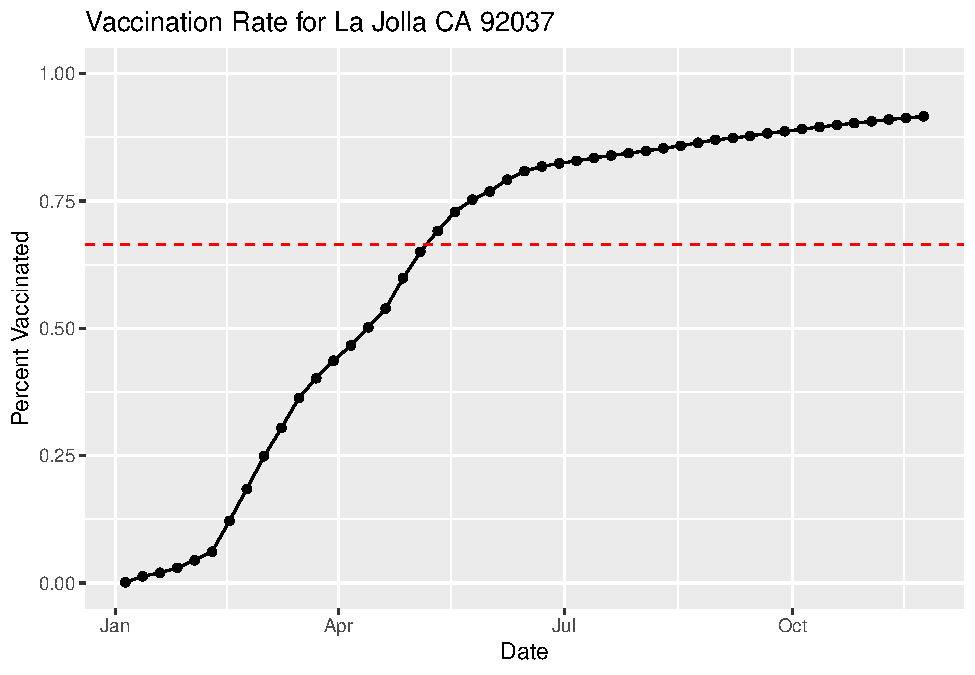
\includegraphics{Class17_files/figure-latex/unnamed-chunk-34-1.pdf}

\begin{quote}
\textbf{Q17}. What is the 6 number summary (Min, 1st Qu., Median, Mean,
3rd Qu., and Max) of the \emph{``Percent of Population Fully
Vaccinated''} values for ZIP code areas with a population as large as
92037 (La Jolla) \emph{as\_of\_date} ``2021-11-16''?
\end{quote}

\begin{Shaded}
\begin{Highlighting}[]
\FunctionTok{summary}\NormalTok{(vax}\FloatTok{.36}\SpecialCharTok{$}\NormalTok{percent\_of\_population\_fully\_vaccinated)}
\end{Highlighting}
\end{Shaded}

\begin{verbatim}
##    Min. 1st Qu.  Median    Mean 3rd Qu.    Max. 
##  0.3529  0.5905  0.6662  0.6640  0.7298  1.0000
\end{verbatim}

\begin{quote}
\textbf{Q18}. Using ggplot, generate a histogram of this data.
\end{quote}

\begin{Shaded}
\begin{Highlighting}[]
\FunctionTok{ggplot}\NormalTok{(vax}\FloatTok{.36}\NormalTok{) }\SpecialCharTok{+} \FunctionTok{aes}\NormalTok{(percent\_of\_population\_fully\_vaccinated) }\SpecialCharTok{+} 
  \FunctionTok{geom\_histogram}\NormalTok{(}\AttributeTok{bins=}\DecValTok{40}\NormalTok{) }\SpecialCharTok{+} \FunctionTok{labs}\NormalTok{(}\AttributeTok{x=}\StringTok{"Percent Vaccinated"}\NormalTok{, }\AttributeTok{y=}\StringTok{"Count"}\NormalTok{)}
\end{Highlighting}
\end{Shaded}

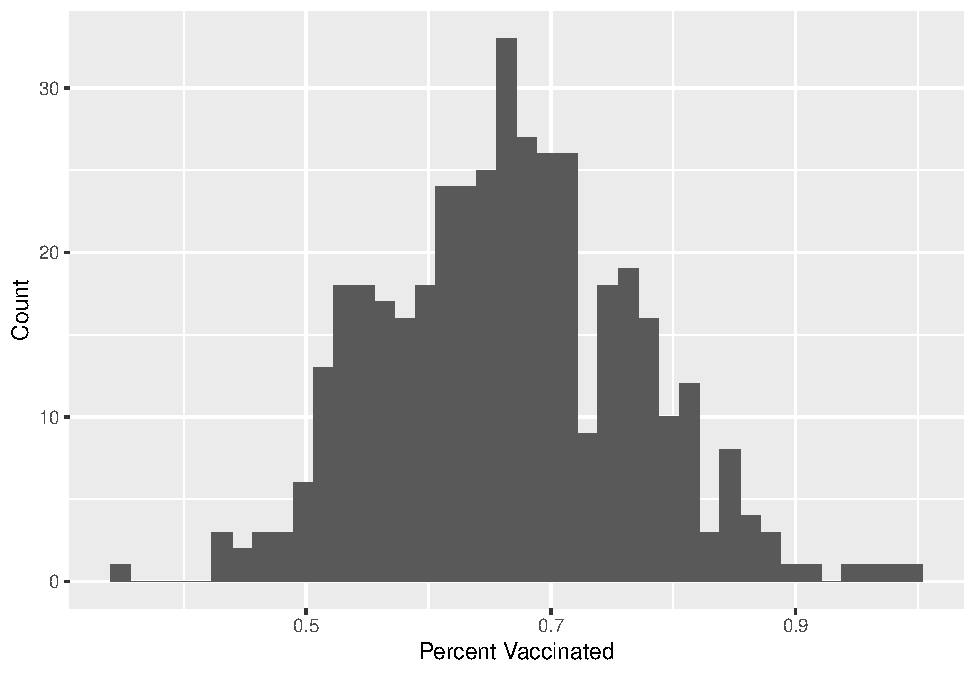
\includegraphics{Class17_files/figure-latex/unnamed-chunk-36-1.pdf}

\begin{quote}
\textbf{Q19}. Is the 92109 and 92040 ZIP code areas above or below the
average value you calculated for all these above?
\end{quote}

\begin{Shaded}
\begin{Highlighting}[]
\NormalTok{vax }\SpecialCharTok{\%\textgreater{}\%} \FunctionTok{filter}\NormalTok{(as\_of\_date }\SpecialCharTok{==} \StringTok{"2021{-}11{-}16"}\NormalTok{) }\SpecialCharTok{\%\textgreater{}\%}  
  \FunctionTok{filter}\NormalTok{(zip\_code\_tabulation\_area}\SpecialCharTok{==}\StringTok{"92109"}\NormalTok{) }\SpecialCharTok{\%\textgreater{}\%}
  \FunctionTok{select}\NormalTok{(percent\_of\_population\_fully\_vaccinated)}
\end{Highlighting}
\end{Shaded}

\begin{verbatim}
##   percent_of_population_fully_vaccinated
## 1                                0.68863
\end{verbatim}

\begin{Shaded}
\begin{Highlighting}[]
\NormalTok{vax }\SpecialCharTok{\%\textgreater{}\%} \FunctionTok{filter}\NormalTok{(as\_of\_date }\SpecialCharTok{==} \StringTok{"2021{-}11{-}16"}\NormalTok{) }\SpecialCharTok{\%\textgreater{}\%}  
  \FunctionTok{filter}\NormalTok{(zip\_code\_tabulation\_area}\SpecialCharTok{==}\StringTok{"92040"}\NormalTok{) }\SpecialCharTok{\%\textgreater{}\%}
  \FunctionTok{select}\NormalTok{(percent\_of\_population\_fully\_vaccinated)}
\end{Highlighting}
\end{Shaded}

\begin{verbatim}
##   percent_of_population_fully_vaccinated
## 1                               0.521047
\end{verbatim}

The 92109 ZIP code area is above the average value of 0.6630. However,
the 92040 ZIP code area is below the average value.

\begin{quote}
\textbf{Q20}. Finally, make a time course plot of vaccination progress
for all areas in the full dataset with a
\texttt{age5\_plus\_population\ \textgreater{}\ 36144}.
\end{quote}

\begin{Shaded}
\begin{Highlighting}[]
\NormalTok{vax.}\FloatTok{36.}\NormalTok{all }\OtherTok{\textless{}{-}} \FunctionTok{filter}\NormalTok{(vax, age5\_plus\_population }\SpecialCharTok{\textgreater{}} \DecValTok{36144}\NormalTok{)}


\FunctionTok{ggplot}\NormalTok{(vax.}\FloatTok{36.}\NormalTok{all) }\SpecialCharTok{+}
  \FunctionTok{aes}\NormalTok{(as\_of\_date,percent\_of\_population\_fully\_vaccinated, }
      \AttributeTok{group=}\NormalTok{zip\_code\_tabulation\_area) }\SpecialCharTok{+}
  \FunctionTok{geom\_line}\NormalTok{(}\AttributeTok{alpha=}\FloatTok{0.2}\NormalTok{, }\AttributeTok{color=}\StringTok{"blue"}\NormalTok{) }\SpecialCharTok{+}
  \FunctionTok{ylim}\NormalTok{(}\FunctionTok{c}\NormalTok{(}\DecValTok{0}\NormalTok{,}\DecValTok{1}\NormalTok{)) }\SpecialCharTok{+}
  \FunctionTok{labs}\NormalTok{(}\AttributeTok{x=}\StringTok{"Date"}\NormalTok{, }\AttributeTok{y=}\StringTok{"Percent Vaccinated"}\NormalTok{,}
       \AttributeTok{title=}\StringTok{"Vaccination Rate Across California"}\NormalTok{,}
       \AttributeTok{subtitle=}\StringTok{"Only areas with a population above 36K are shown."}\NormalTok{) }\SpecialCharTok{+}
  \FunctionTok{geom\_hline}\NormalTok{(}\AttributeTok{yintercept=}\FloatTok{0.66}\NormalTok{, }\AttributeTok{linetype=}\StringTok{"dashed"}\NormalTok{)}
\end{Highlighting}
\end{Shaded}

\begin{verbatim}
## Warning: Removed 176 row(s) containing missing values (geom_path).
\end{verbatim}

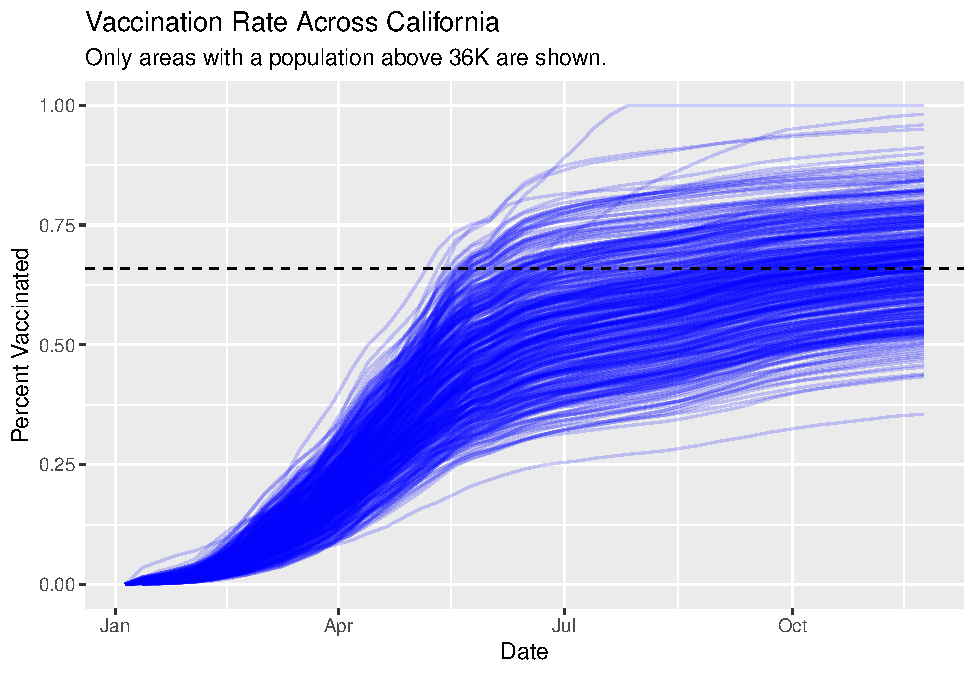
\includegraphics{Class17_files/figure-latex/unnamed-chunk-38-1.pdf}

\begin{quote}
\textbf{Q21}. How do you feel about traveling for Thanksgiving and
meeting for in-person class next Week?
\end{quote}

With the detection of the omicron variant, which is more transmittable
than the delta variant, and the combination of the lower-than-expected
vaccination rates uncovered in this activity, I feel hesitant about
meeting for in-person class next week. Traveling by car is safe enough,
but traveling by plane for Thanksgiving is slightly concerning to me.

\end{document}
